\section{git}

\begin{frame}
  \tableofcontents[currentsection]
\end{frame}

\begin{frame}{Installation}
  \begin{itemize}
    \item Linux:
    \begin{itemize}
      \item Debian, Ubuntu: \texttt{[sudo] apt-get install \textit{git-core}}
      \item Arch: \texttt{[sudo] pacman -S \textit{git}}
    \end{itemize}
    \item Windows:
    \begin{itemize}
      \item MySysGit: \url{http://code.google.com/p/msysgit}
      \item TortoiseGit: \url{http://code.google.com/p/tortoisegit}
    \end{itemize}
    \item Mac:
    \begin{itemize}
      \item Git for OS X: \url{http://code.google.com/p/git-osx-installer}
    \end{itemize}
  \end{itemize}
\end{frame}

\begin{frame}[fragile]{initiale Konfiguration}
  \begin{itemize}
    \item Identität festlegen:
    \begin{lstlisting}
$ git config --global user.name "John Doe"
$ git config --global user.email johndoe@example.com
    \end{lstlisting}
    \item Editor festlegen (optional):
    \begin{lstlisting}
$ git config --global core.editor whatever
    \end{lstlisting}
    \end{itemize}
\end{frame}

\begin{frame}{Die möglichen Zustände einer Datei}
  \begin{columns}
    \begin{column}{0.45\textwidth}
      \begin{figure}
        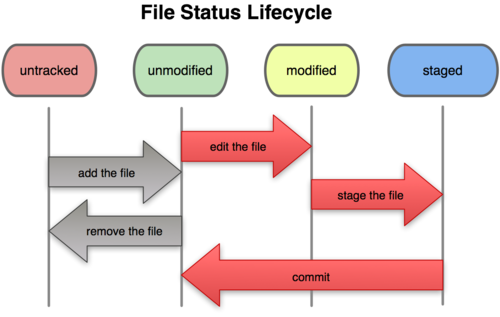
\includegraphics[width=\textwidth]{img/file_lifecycle}
        \caption[format=empty]{Quelle: \url{http://progit.org}}
      \end{figure}
    \end{column}
    \begin{column}{0.65\textwidth}
      \begin{itemize}
        \item nicht versioniert (\textbf{untracked})
        \item versioniert, aber unverändert (\textbf{unmodified})
        \item versioniert und verändert (\textbf{modified})
        \item versioniert, verändert und in der „staging area“ (\textbf{staged})
      \end{itemize}
    \end{column}
  \end{columns}
\end{frame}

\begin{frame}[fragile]{typischer Workflow}
  \begin{itemize}
    \item Initialisieren eines git Repositories
    \begin{lstlisting}
$ cd meinprojekt
$ git init
    \end{lstlisting}
    \item Dateien der „staging area“ hinzufügen
    \begin{lstlisting}
$ git add <file>
    \end{lstlisting}
    \item Änderungen der „staging area“ committen
    \begin{lstlisting}
$ git commit -m 'initial commit'
    \end{lstlisting}
    \end{itemize}
\end{frame}

\begin{frame}[fragile]{Änderungen betrachten}
  \begin{itemize}
    \item Den aktuellen Status des Repositories betrachten
    \begin{lstlisting}
$ git status
    \end{lstlisting}
    \item Änderungen im Arbeitsverzeichnis betrachten
    \begin{lstlisting}
$ git diff
    \end{lstlisting}
    \item Änderungen betrachten, die sich bereits in der „staging area“ befinden
    \begin{lstlisting}
$ git diff --cached
    \end{lstlisting}
  \end{itemize}
\end{frame}

\begin{frame}[fragile]{Tipps und Tricks}
  \begin{itemize}
    \item keine temporären Dateien in das git Repository aufnehmen
    \begin{itemize}
      \item erschwert das effiziente Arbeiten mit git
      \item bläht das Repository unnötig auf
    \end{itemize}
  \end{itemize}
  \lstset{frame=single}
  \begin{lstlisting}[caption=Inhalt der Datei .gitignore]
*.swp       #alle swp Dateien
doc/*.aux   #alle aux Dateien im Verzeichnis doc/
tmp/**/*    #alle Dateien im Verzeichnis tmp/
  \end{lstlisting}
\end{frame}

\begin{frame}[fragile]{Tipps und Tricks}
  \begin{itemize}
    \item „gute“ commit messages \ldots
    \begin{itemize}
      \item vereinfachen die Zusammenarbeit
      \item ermöglichen das schnelle Verfolgen von Änderungen
    \end{itemize}
  \end{itemize}
  \begin{lstlisting}[frame=single,caption={Quelle: \url{http://tbaggery.com/2008/04/19/a-note-about-git-commit-messages.html}}]
Short (50 chars or less) summary of changes

More detailed explanatory text, if necessary.  Wrap it to about 72
characters or so.  In some contexts, the first line is treated as the
subject of an email and the rest of the text as the body.  The blank
line separating the summary from the body is critical (unless you omit
the body entirely); tools like rebase can get confused if you run the
two together.
  \end{lstlisting}
\end{frame}

% vim: tabstop=2 expandtab shiftwidth=2 softtabstop=2 autoindent
